\chapter{Design and design notes}

\section{Actuator selection}
There is many different types of actuators used in exoskeletons. The most common once are pneumatic, hydraulic and electrical \citep{maciejasz2014survey}. Hydraulic actuator is commonly used for high power application such as military and industrial lifting. Electrical motors is the most popular actuator in the field of rehabilitation. This is mainly due to it high controllability and high position accuracy. Light weight batteries can be used as the energy source providing flexible and mobile systems. [ROBOT Book]

To be able to select an appropriate motor, several factors need to be evaluated. The most important is the torque force(Unknown) and speed (>2.066 rad/s | > 120deg/s), then the weight, size and the price.

(Servo vs stepper vs dc motor) 

Linear transition? 

\subsection{Actuator for this thesis}
Since this project is based on a previous one, some motors have all ready been purchased and tested. And since the accurate value for the needed torque is hard to obtain, the MX-28 motor will be used for the first prototype. From the litterateur it can be found that the muscle reflex can provide everything between. 


\section{Sensor selection}
1. Dynamic, 2. Kinematic, 3. Trigger signals. 
Most exoskeleton require a some sensor feedback to control the force, torque and angle of the device, and some actuators has these sensors integrated. But since the link between the body and the device usually is not absolutely rigid, additional sensors can be used to improve the system response time [Thomas]. This is especially critical for person-in-control applications where the user should not experience any resistance from the device. Thomas Evison and others [kilder] have used dynamic signals to improve the performance of the controller by measuring the instant change of movement and use it as the controller input. It has been proven that such a closed loop controller can significantly decrease the system impedance. Some commonly used sensors is load-cells, EMG sensors and force sensors. 

Kinematic signal is also important for accurate position control.
With sensor is the best suited for angular measuremnt.
 \textcolor{red}{TODO}

\subsection{This thesis}
For this thesis the MX-28 electrical motor is likely to be used. This has all ready an potenitimeter implemented. 



\section{Control}



\section{Design method}
% Soft vs Rigid
One of the major challenges in exoskeleton development is weight.  Hence, it is important to select the correct material. Depending on the application, the materials used in such devices vary. One way of designing exoskeletons is with a soft bodies. These designs have the advantage of being light weighted and comfortable to wear \cite{sEMG-based2019, lu2019development, sridar2017development}. However, it is hard to attach actuators and sensors to the soft exoskeleton it self, and consequently the complexity of the system will increase. Another and more common way of design is the rigid exoskeletons. It is usually made with a steel, aluminium, titanium or carbon fibre body to make it strong and stable. Titanium and carbon fibre provides the best strength-to-weight ratio, but it is more expensive than the others. Therefore, aluminium is the most popular choice since it has a relatively good weight-to-strength ratio and is fairly cheap. For being able to attach the device to the human body, plastic or similar material is used to provide a flexible fit of the exoskeleton. [Kilde] 

\subsection{Material}
Compare PLA, ABS And Carbon filament in therms of flexibility, durability and strength.


\begin{table}[h!]
\centering
\begin{tabular}{|c|c|}
\hline
\textbf{Application} & \textbf{Material} \\ \hline
Joint/Frame & Aluminum \\ \hline
Fit prototype & Plastic (ABS) \\ \hline
Fit later design & Carbon? \\ \hline
Comfort & Neoprene? \\ \hline
\end{tabular}
\end{table}

\section{Notes and summaries}
\begin{itemize}
    \item Electric actuators will be used due to it angular accuracy. 
    \item 
    \item 
\end{itemize}{}


\section{Design measurements}
According to ANTHROPOMETRY AND MASS DISTRIBUTION FOR HUMAN ANALOGUES, the different average measurement of different body parts is: 
\begin{table}[h!]
\centering
\begin{tabular}{|c|c|c|c|}
\hline
\textbf{Body part} & \multicolumn{3}{c|}{\textbf{Measurement (mm)}} \\ \hline
Size & S & M & L \\ \hline
Forearm Circumference & 265 & 285 & 302 \\ \hline
Upper Arm Circumference & 284 & 313 & 337 \\ \hline
Wrist Circumference & 167 & 177 & 187 \\ \hline
Forearm Length &  &  &  \\ \hline
Upper arm langth &  &  &  \\ \hline
\end{tabular}
\end{table}



\section{Actuation method and transition}
Research pros and cons of belt driven, gear and 

https://www.jospt.org/doi/pdf/10.2519/jospt.1997.25.6.395 \newline

https://itstillruns.com/calculate-gear-ratios-torque-8140164.html \newline

\section{Evaluation of previous design}


\section{Elbow Torque and Angular Velocity}
\subsection{Bio dynamics Founder}
Hill model: 

\subsection{Reffs}
\begin{enumerate}
    \item Monitoring elbow isometric contraction by novel wearable fabric sensing device.
\end{enumerate}{}
\begin{figure}[h!]
    \centering
    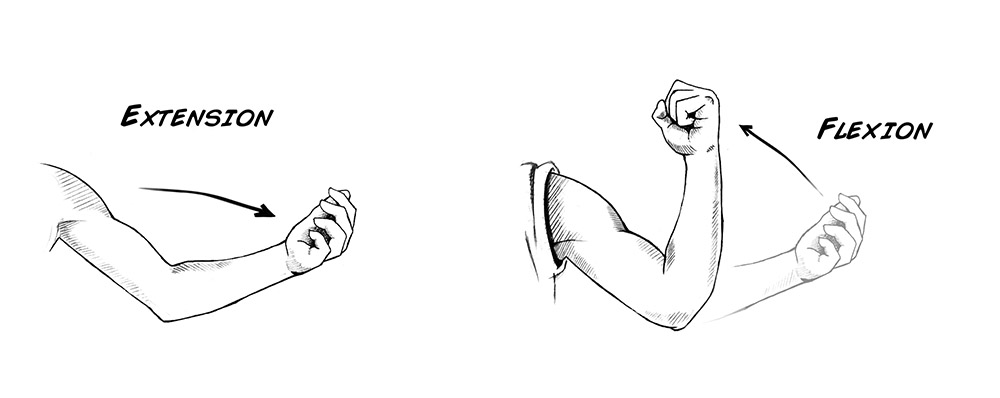
\includegraphics{compact-template/Fig/flexextend.jpg}
    \caption{Flexion and Extraction}
    \label{fig:flexextend}
\end{figure}{}


\section{Balance and recovery research}
\subsection{Center of pressure (COP)}
\textcolor{blue}{TO READ LATER} \newline
In the book Proximal-to-Distal Sequencing Behavior chapter 10, the theory of center of pressure (COP) is explained. This talks about how the human body transfers pressure to the ground to keep balanced. In addition this chapter contains an MatLab example of how to calculate the center of gravity for a moving body based on the measurements from a force plate. 

